
\section{Possible cobot Solutions} \label{ch:UR}

This section is taking 2 different cobots in to consideration for a possible solution to the case description.

\subsection{UR}

Universal Robots was founded in 2005 by a group of Danish engineers. Their thought was, that every industrial robot on the market was designed to be big, heavy and expensive. Therefore the group decided to make a smaller and more agile kind of industrial robot.\cite{Urhist}\\


The UR is now being used to several different repetitive tasks by big and small companies.
Because UR robots are much smaller and do not have the same force as their bigger counterparts, they can be used in cooperation with humans, which is one of the biggest advantages. This allows the robots to be much more flexible and manageable.\\



These robots can work with humans, and are called collaborative robots/cobots.\\
Here are the specification for the UR5:\\ 

\subsubsection{UR5}

\begin{figure}[h]
    \centering
    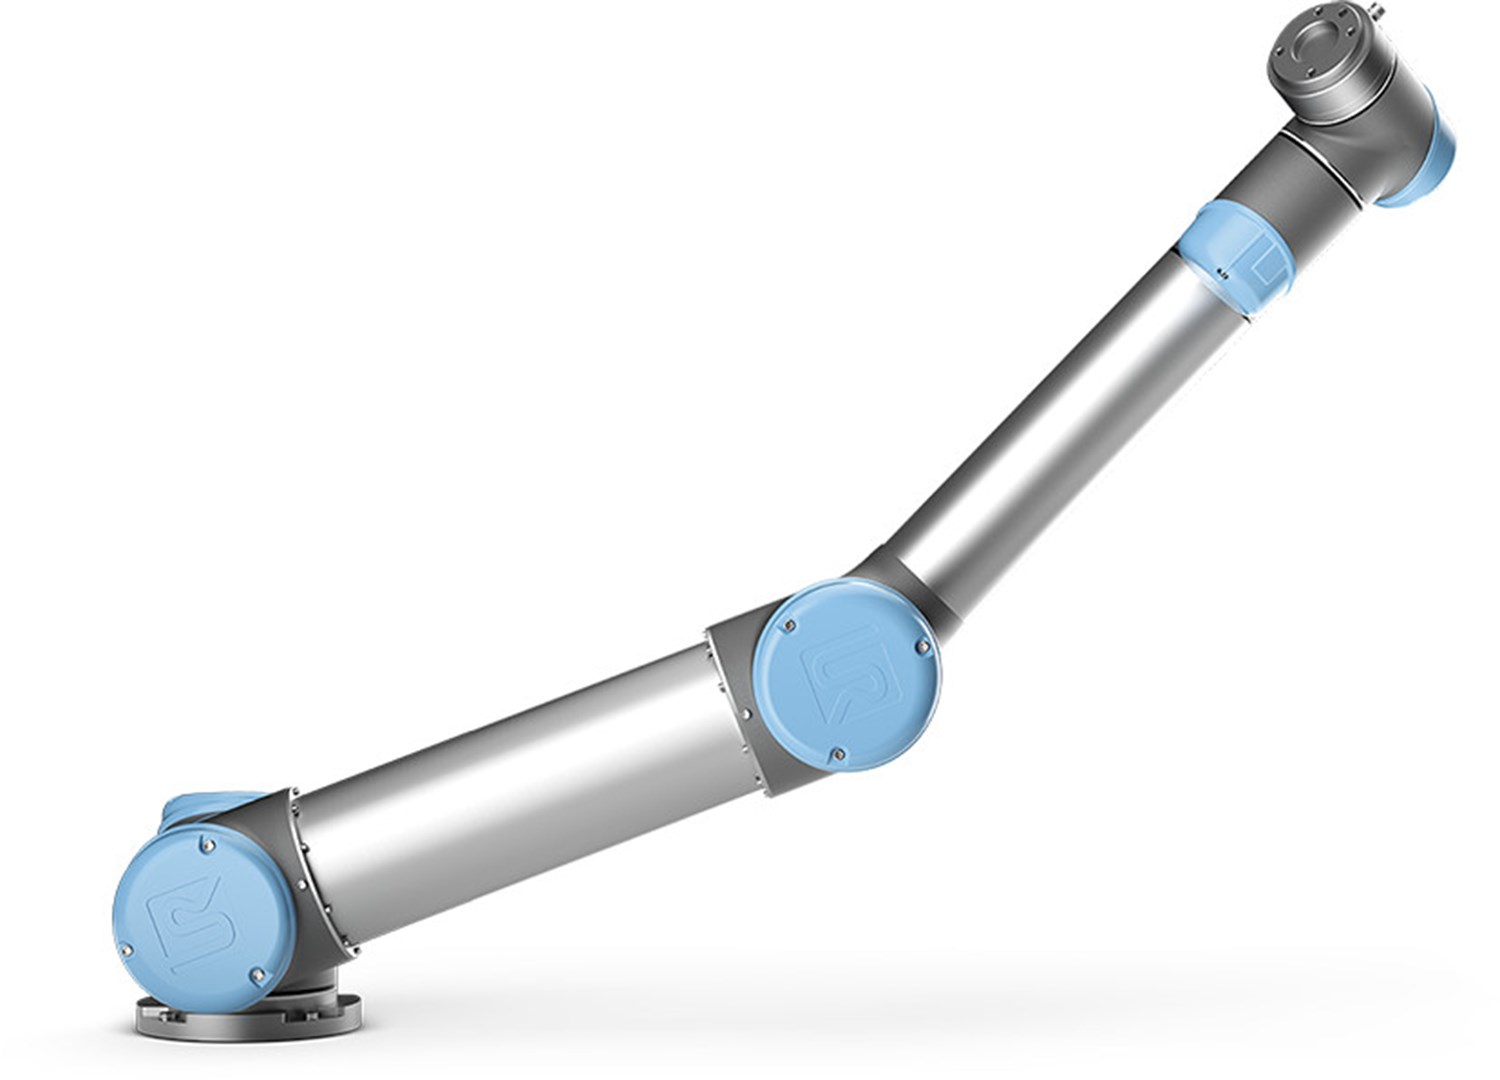
\includegraphics[width=9cm]{UR/UR5pic.jpg}
    \caption{Universal Robots UR5 \cite{UR5billede}}
    \label{fig:UR5}
\end{figure}

\begin{itemize}
    \item Weight: 18.4 kg.
    \item Payload: 5 kg.
    \item Footprint: 149 mm.
    \item Joints: +/-360 degrees on all the joints.
    \item Operating life: 35,000 Hours.
    \item Speed: joints = 180 degrees/sec, tool = 1 m/sec.
    \item Reach: 850 mm.
    \item Repeatability: +/- 0.1 mm.
\end{itemize}
The materials used on all the cobots are aluminum and plastic\cite{Ur5_about}\cite{UR5_tech}.


\subsubsection{KUKA}

The KUKA company started more than a hundred years ago. They were the first to invent point welding gripper in Germany.\\
As the years goes by the KUKA company writes history by inventing the world first industrial lightweight robot with sensors in every axis.\\

KUKA and UR are competitors since they have the same market, hence is why this project will take both in to consideration of a possible optimization of the work-cell\cite{KukaHist}.\\


\subsubsection{KUKA LBR IIWA 7 R800}
\begin{figure}[h]
    \centering
    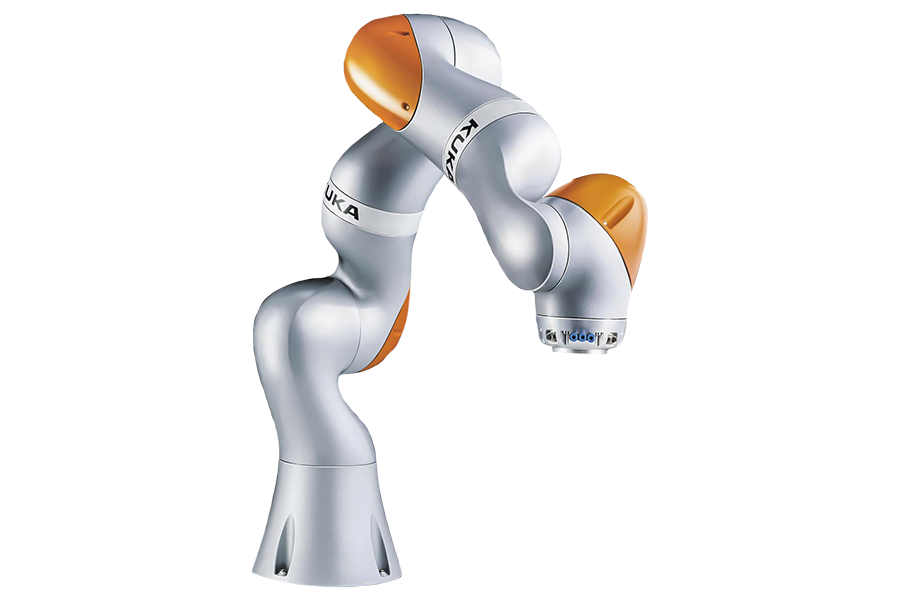
\includegraphics[width=9cm]{UR/1502895088_1.png}
    \caption{KUKA LBR IIWA 7 R800 \cite{KUKAbillede}}
    \label{fig:LBR IIWA}
\end{figure}

Here are the specification for the LBR iiwa 7 R800:\\

\begin{itemize}
    \item Weight: 23.9 kg.
    \item Payload: 7 kg.
    \item Footprint: 136 mm.
    \item Joints: Ranging from +/-120 degrees to +/-170.
    \item Operating life: 30,000 Hours.
    \item Speed: Joints = 180 degrees/sec
    \item Reach: 800-820 mm
    \item Repeatability: +/- 0.1 mm.
\end{itemize}
\cite{KukaSpec1},\cite{KukaSpec2}.

\subsection{Why cobots?}\label{ch:Whycobot}
Why is there a need for a cobot? A thing that is mentioned in an article about cobots, in an assembly line, is that cobots can help reduce the ergonomics stress level of the employees\cite{Coboau}. Another way this can help the production flow, is that the robot can preform some tedious task while the employee can take care of the complex tasks in the work area.\\

\subsection{Which cobot is more suitable?}

Having the case description in mind \ref{ch:case description}, and the fact that the process must not be more than 26 seconds, before a fully functional rotor is ready.\\
The cobots have almost similar specifications, the only major difference is the rotations of the joints. In this case a huge maneuverability is required, hence the rotation of the joints is a factor weighed highly in this process. Beside that, the only difference would be what would suit the company the most. Since Grundfos has implemented KUKA's is because it is easier to run a production-line with the same system, and the workers know these robots.\\
The most suitable for this project is UR5.

\subsection{Conclusion}

%Taking all of the above into consideration, some data can be included in the ideal robot for this case.\\ 
%Having an overview of the different tasks that has to be preformed and using the tools that are given, the project can get closer to a conclusion for the robot.\\
%The project has focused on two different cobots, 1 from KUKA, and 1 from UR. They are then set up to conclude which has the better specifications. By looking at nothing else than the specifications, the most suitable for this case is the UR5.\\

\newpage

